\section{Requisitos}
Este capítulo describe cómo organizar y grabar un CD de audio compatible con Red Book. Traverso usa \texttt{cdrdao} para grabar el CD, por tanto éste programa debe estar instalado. \texttt{cdrdao} está disponible en la mayoría de los repositorios de las distribuciones Linux actuales. Se recomienda por tanto instalarlo usando el gestor de paquetes de su distribución. El instalador para Windows y Mac se ocupa él mismo de instalar cdrdao, así que si usa una de éstas plataformas, puede obviar esta sección.

\footnotesize
\begin{verbatim}
tux@linux:~$ cdrdao

Cdrdao version 1.2.2 - (C) Andreas Mueller <andreas@daneb.de>
  SCSI interface library - (C) Joerg Schilling
  Paranoia DAE library - (C) Monty

Check http://cdrdao.sourceforge.net/drives.html#dt for current 
driver tables.


Usage: cdrdao <command> [options] [toc-file]
command:
...
\end{verbatim}
\normalsize

Instalar \texttt{cdrdao} en Linux es inmediato, ya que forma parte de casi todas las distribuciones. Abra el gestor de paquetes de su distribución, busque \texttt{cdrdao} e instale el binario correspondiente.

\section{Pistas y Marcadores}
Hay dos formas de definir pistas para un CD. Cada hoja puede ser una pista, o bien puede hacerse que la linea de tiempo de una hoja se corresponda con el CD completo. En el último caso, los marcadores delimitan las pistas del CD. También es posible combinar ambos procedimientos. Seguidamente se detallan estos conceptos

\subsection{Cada hoja es una pista del CD}
Como habrá apreciado, Traverso permite que existan varias hojas en un proyecto. A mucha gente le gusta esto, porque les permite combinar todas las hojas de un álbum en un proyecto, sin impedirles centrarse en una particular. Si quiere grabar un CD que contenga todas las hojas de un proyecto, asegúrese de marcar el botón ``Todas las Hojas'' en la ventana de exportación. Cada hoja se grabará como una pista del CD.

\subsection{El CD a partir de una línea de tiempo}
A veces es importante ajustar con detalle la transición de una pista a la siguiente, por ej., añadiendo un pequeño silencio entre medias, o haciendo desaparecer una mientras aparece la siguiente. En estos casos es mejor disponer todo el CD en una línea de tiempo y separar las pistas mediante marcadores. Veamos un ejemplo (consulte la \FigT~\ref{fig_markers01} si se pierde en las explicaciones). Abra o cree un proyecto con sólo dos clips de audio. Asuma que el clip 1 será la pista 1 del CD, y el clip 2 la pista 2. Colóquelos por ejemplo en la primera y segunda pistas, respectivamente, comenzando el primero en la posición 00:00:00, como esperaría que ocurriera en el CD. Deje un pequeño silencio entre el final del primer clip y el comienzo del segundo. Para que Traverso comience aquí la segunda pista, desplace el ratón hasta el silencio, y pulse \sact{M}. Esto añade un pequeño triángulo (marcador) en la línea de tiempo, en la posición del ratón, y otros dos más, uno en la posición 00:00:00 y otro en el final del clip 2. El último tiene la etiqueta ``End'', y marca el final del CD. Puede moverlo un poco a la derecha si no quiere que el CD acabe aquí (puede ser que haya colas de reverb, que no querrá cortar).

\begin{figure}[t]
 \centering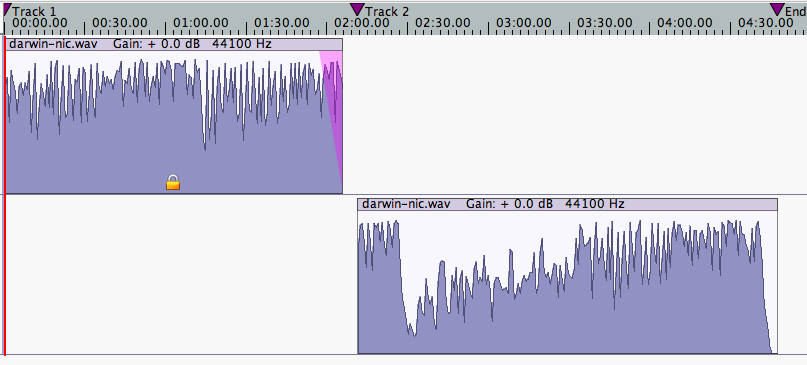
\includegraphics[width=\textwidth]{../images/markers01}
 \caption{Si un CD se dispone en una hoja, los marcadores definen la separación entre pistas. No borre los marcadores de 00:00:00 y del final.}
 \label{fig_markers01}
\end{figure}

Los triángulos actúan como marcadores de pista del CD, y pueden ser añadidos, movidos o borrados libremente (pulse \sact{Q} sobre la línea de tiempo para ver las funciones disponibles). Pero también se puede crear disposiciones que no tengan sentido, por ejemplo un sólo marcador en la línea de tiempo. En estos casos, Traverso trata de adivinar la disposición más razonable, y añade marcadores en concordancia (usualmente en 00:00:00 y tras el último sample de audio que exista en la hoja). Traverso admite también texto de CD, que puede introducirse en ``Hoja $\rightarrow$ Editor de Marcadores\dots'' (\FigB~\ref{fig_marker-editor}). También es posible exportar desde ésta ventana la tabla de contenidos del CD como un fichero HTML. El texto de CD relativo a todo el álbum puede introducirse en los ajustes de proyecto, al que se accede desde ``Proyecto $\rightarrow$ Administrar Proyecto'', en la pestaña ``Texto de CD''.

\begin{figure}[ht]
 \centering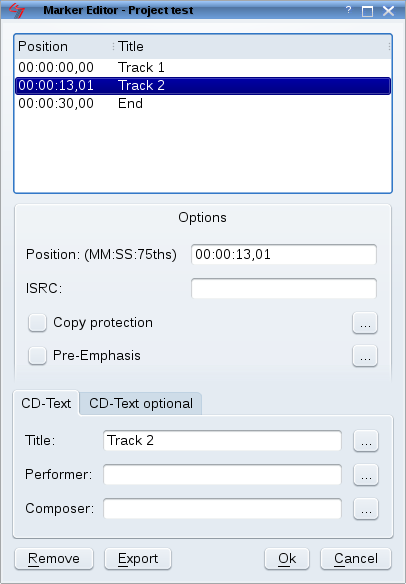
\includegraphics[width=0.4\textwidth]{../images/marker-editor}
 \caption{La ventana de marcadores, que se abre en ``Hoja $\rightarrow$ Editor de Marcadores\dots'' permite añadir texto de CD, modificar los marcadores, y exportar la tabla de contenidos como archivo HTML.}
 \label{fig_marker-editor}
\end{figure}

Cuando el proyecto esté a su gusto, pulse \sact{F8} o vaya a ``Proyecto $\rightarrow$ grabar CD\dots'' para abrir la ventana de grabación del CD (\FigB~\ref{fig_exportdlg}). Debe decidir ahora si grabará la hoja activa (los marcadores definirán las pistas del CD) o el proyecto entero (cada hoja será una pista del CD). Si marca ``Sólo exportar a disco'', no se grabará un CD, sino que se creará un archivo *.toc y los archivos *.wav para \texttt{cdrdao}.

Para exportar la hoja o el proyecto al disco duro, pulse \sact{F9} o seleccione ``Proyecto $\rightarrow$ Exportar\dots'' del menú. Esto abre otra ventana (\FigB~\ref{fig_exportdlg}), donde puede elegir el formato de archivo, y ajustar varios parámetros. Traverso proporciona los tipos de archivo más comunes, incluyendo Wave, AIFF, FLAC, WavPack, Ogg Vorbis, y MP3. Si uno o más formatos no están disponibles en su sistema, Probablemente Traverso fue compilado sin soporte para ellos. Algunas distribuciones prefieren no incluir soporte para ciertos formatos comprimidos debido a razones legales. En ese caso, puede conformarse con ello, o compilar Traverso usted mismo con soporte para el codec en cuestión.

Nota para usuarios de OS X: el soporte para grabación de CD es aún experimental. Puede elegir entre varios dispositivos de grabación: IODVDServices, IODVDServices/2, IOCompactDiscServices, IOCompactDiscServices/2. Están programados en el sistema, y probablemente usted no tenga todos ellos disponibles. IOCompactDiscServices sólo debiera usarse para lectores antiguos sin capacidad de lectura de DVD. Si dispone de varias unidades de DVD, use IODVDServices o IODVDServices/2 para acceder a la primera o segunda unidad. En muchos casos IODVDServices será lo único que funcione.

\begin{figure}[t]
 \centering
 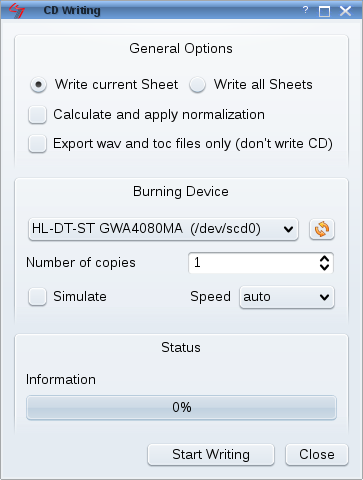
\includegraphics[width=0.35\textwidth]{../images/exportdlg}\qquad
 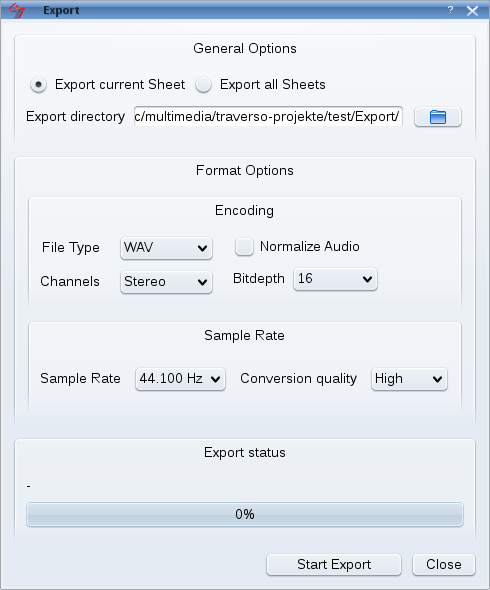
\includegraphics[width=0.45\textwidth]{../images/exportdlg1}
 \caption{\sact{F8} abre una ventana que permite grabar la hoja activa o el proyecto entero en un CD (izda.)  \sact{F9} abre una ventana de exportación de la hoja activa o del proyecto entero al disco duro (dcha.)}
 \label{fig_exportdlg}
\end{figure}

